\section{Implementation and Deployment}
We have deployed \name on \company's DCs, which consist of dozens of IDCs located in three major regions in China. \name is implemented with 3621 lines of golang code \cite{golang}, and can be fully integrated in \company's DCs.

Figure \ref{fig:implementation} shows the detailed implementation of \name. It  consists of five components: \emph{Controller}, \emph{Agent Monitor}, \emph{Agent}, \emph{Storage Platform}, \emph{Network Monitor}. 1) \emph{Controller} is a scheduler which executes the customized scheduling algorithm. 2) \emph{Agent Monitor} delivers messages between the \emph{Controller} and \emph{Agent}. 3) \emph{Agent} is a module deployed in each machines. It announces the bulk data that need to be downloaded to \emph{Agent Monitor}. 4) \emph{Network Monitor} records the each link capacity and the traffic of latency-sensitive data, which is the basic input of the scheduling algorithm. 5) \emph{Storage platform} records the system snapshot, including master and slave status, etc. The \emph{Controller} is replicated three times for fault tolerance. Once the master controller fails, the \emph{Storage Platform} will announce one slave becomes the master.

The basic workflow of \name can be described as follows: All the \emph{Agent} sends its task and status to \emph{Agent Monitor} by HTTP POST, then \emph{Agent Monitor} aggregates all information for \emph{Controller} to perform scheduling. Once scheduling is finished. \emph{Agent Monitor} send the control message to all the \emph{Agent} by HTTP POST, then \emph{Agent} uses \emph{wget} tools to download bulk data. After one scheduling cycle (\fillme), the above procedure will performed again.

Note that only \emph{Agent} is deployed in each IDC's machines, the other components is deployed in centralized clusters, so \name can be easily deployed to other companies' DCs.
	
\begin{figure}[htbp]
  \centering
  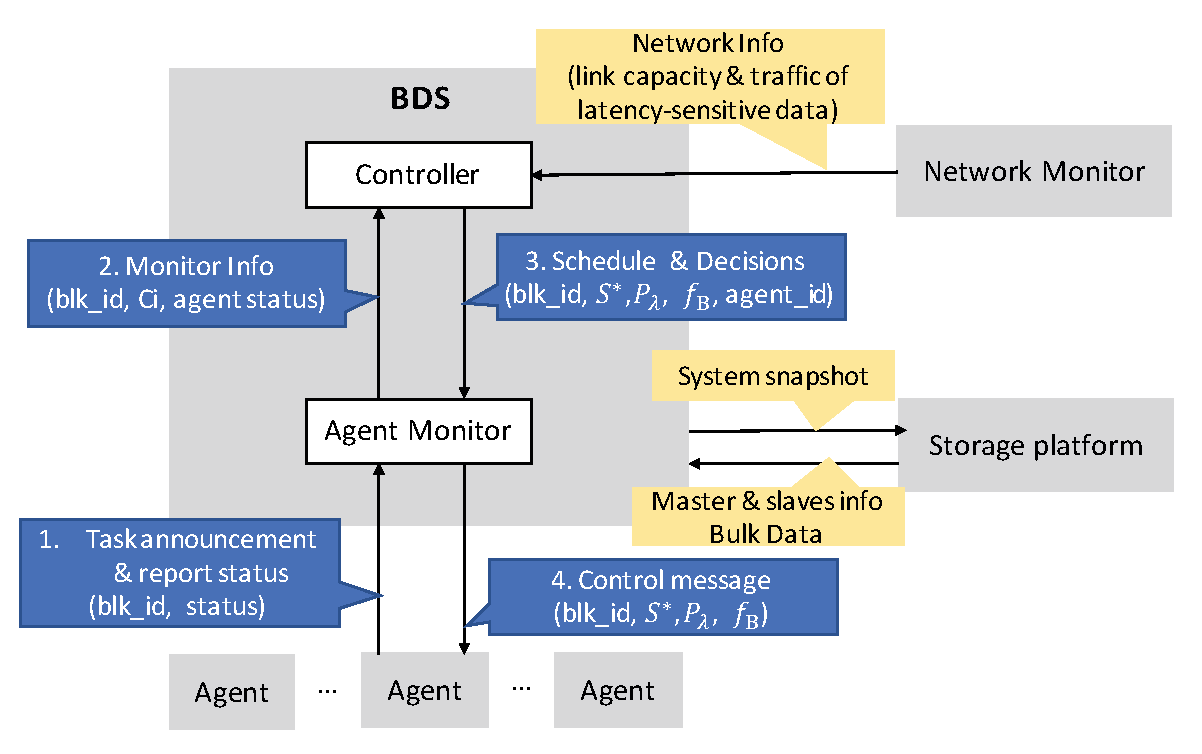
\includegraphics[width=3in]{images/implementation.eps}
  \caption{The implementation of \name.}
  \label{fig:implementation}
\end{figure}
\vspace{-15pt}

%
%\begin{itemize}
%\item \name consists of \fillme line of \fillme code, and can be fully integrated in \company's DCs.
%
%\item Application interfaces: What information does an application need to announce to \name to initiate a multicast.
%
%\item What's the software platform to implement each component
%
%\item Why \name is also applicable to other DCs?
%
%\end{itemize}

